\documentclass[pdf, aspectratio=169]{beamer}
\mode<presentation>{}

\usepackage{amsmath}
\usepackage{amssymb}                 
\usepackage{tikz}
\usetikzlibrary{calc}
\usepackage{graphicx}

\usepackage{bm}

\usepackage{pdfpages}

%defs
\newcommand\pinfeq{\mathrel{\overset{\makebox[0pt]{\mbox{\normalfont\tiny\sffamily inf. p}}}{=}}}

%% preamble
\title{Dissecting the clonal origins of childhood acute lymphoblastic leukemia by single-cell genomics}
\subtitle{Charles Gawad, Winston Koh and Stephen R. Quake}
\author[shortname]{Pandu Raharja}
\institute[shortinst]{Technische Universit\"at M\"unchen\\
Ludwig-Maximillians-Universit\"at M\"unchen}
\date{\today}


\setbeamertemplate{footline}[text line]{%
  \parbox{\linewidth}{\vspace*{-8pt} \hfill  \hfill\insertpagenumber}}
\setbeamertemplate{navigation symbols}{}

\begin{document}

%% title frame
\begin{frame}
\titlepage
\end{frame}

\begin{frame}
	\begin{itemize}
	\item Gawad, Charles, Winston Koh, and Stephen R. Quake. "Dissecting the clonal origins of childhood acute lymphoblastic leukemia by single-cell genomics." Proceedings of the National Academy of Sciences 111.50 (2014): 17947-17952.
	\end{itemize}
\end{frame}

\begin{frame}{Outline}
	\begin{itemize}
		\item Motivation
		\item Methods (+ Results)
		\item Code session
		\item Discussion 
	\end{itemize}
\end{frame}

\begin{frame}{Tumor Heterogeneity\footnotemark}
	\begin{itemize}
		\item \textbf{Cancer} -- a generic term for cells with uncontrolled growth:
		\begin{itemize}
			\item Carcinoma: epithetlial origin
			\item Leukemia: bone marrow origin
			\item Lymphoma: lymph node origin
			\item Sarcoma: connective tissue origin
			\item \textit{and others}
		\end{itemize}
		\item Each class is further divided into multiude of categories
		\item Each category has its own morphological, metabolic, genetic and growth characteristics
	\end{itemize}
\footnotetext[1]{or \textit{why is it almost impossible to "cure" cancer?}}
\end{frame}

\begin{frame}{Tumor Heterogeneity}
	\begin{itemize}
		\item Concerted efforts have been done to map mutational landscape of major cancer classes
		\item (TCGA consortium) Kandoth, Ding \textit{et al} , Nature, 2013:
		
		"\textit{The Cancer Genome Atlas (TCGA) has used the latest sequencing and analysis methods to identify somatic variants across thousands of tumours...Here we present data...3,281 tumours across 12 tumour types...we identified 127 significantly mutated genes...and emerging...cellular processes in cancer...[A]verage number of mutations...varies across tumour types...Mutations in transcriptional factors/regulators show tissue specificity, whereas histone modifiers are often mutated across several cancer types}"		
		
		\item \textbf{TL;DR:} cancer is a damn complex class of diseases
	\end{itemize}
\end{frame}

\begin{frame}{Intratumor Heterogeinity}
	\begin{itemize}
		\item Cancer is mostly born out of series of mutation and epigenetic changes
		\item These changes are inherited along the lineage
		\item New mutation happening in subpopulation create a new clone
	\end{itemize}
	\begin{figure}
		\center
		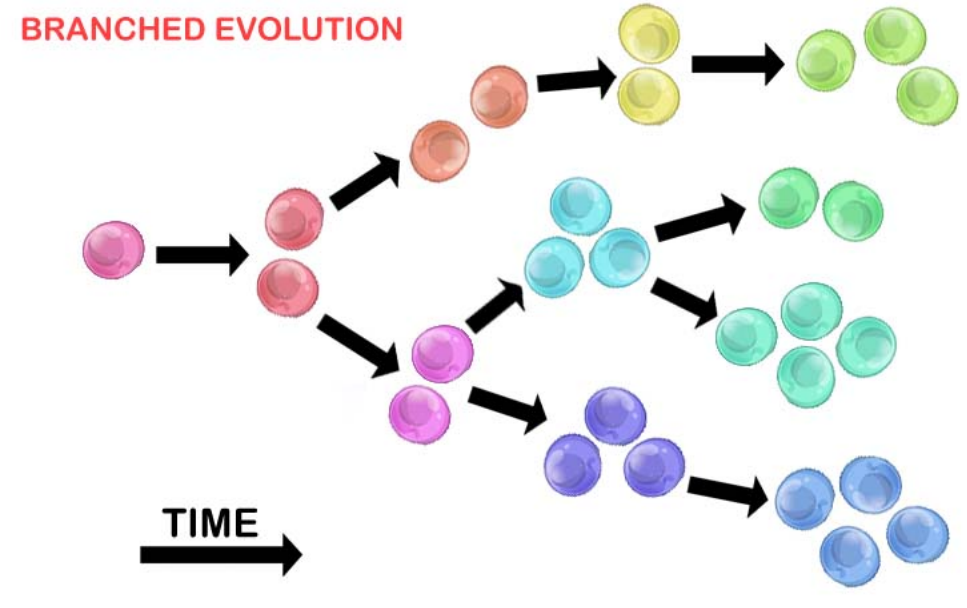
\includegraphics[scale=.3]{02.png}
		{\tiny wikipedia}
	\end{figure}
\end{frame}

\begin{frame}{Intratumor Heterogeinity and Cancer Treatment}

	\begin{figure}
		\center
		
\includegraphics[scale=.3]{01.png}
		{\tiny \,Swanton, Nature, 2012}
	\end{figure}
\end{frame}

\begin{frame}{This paper's motivation}
	\begin{itemize}
		\item Study the dynamics of intratumor heterogeinity:
		\begin{itemize}
			\item Determination of segretation pattern of tumor clones
			\item Reconstruction of clonal tree
			\item Identification of common features across clones
			\item Discovery of proliferative oncogenic point mutations
			\item \textit{etc}
		\end{itemize}
		\item Provide high resolution dynamics of cancer development (in this case, \textit{acute lymphoblastic leukimia (ALL))}
	\end{itemize}
\end{frame}

\begin{frame}{Methods}
	\begin{itemize}
		\item Single-cell cancer genome sequencing protocol
		\item Computational methods to segregate leukimia into distinct clonal populations using combined:
		\begin{itemize}
			\item \textbf{Expectation-Maximization (EM)} on \textbf{multivariate Bernoulli model} with \textbf{AIC} regularization followed by \textbf{Multiple Correspondence Analysis}, AND
			\item \textbf{Clustering} of  mutations using \text{Jaccard distance} with clone number estimation using \textbf{sum of square error} 
		\end{itemize}
		followed by clone tree reconstruction using \textbf{minimum spanning tree reconstruction} on consensus data 
	\end{itemize}
\end{frame}

\begin{frame}{Single-cell cancer genome sequencing}
	\textbf{Main goal:} identify single-cell variants to be used in further analysis
	\begin{itemize}
		\item Bulk Exome Sequencing was conducted to establish reference sequence
		\item Resequencing of each cell (microfluidic cell isolation and sequencing) to identify cell-specific variants
		\item Removal of low quality cells
	\end{itemize}
	
	\begin{figure}
		\center
		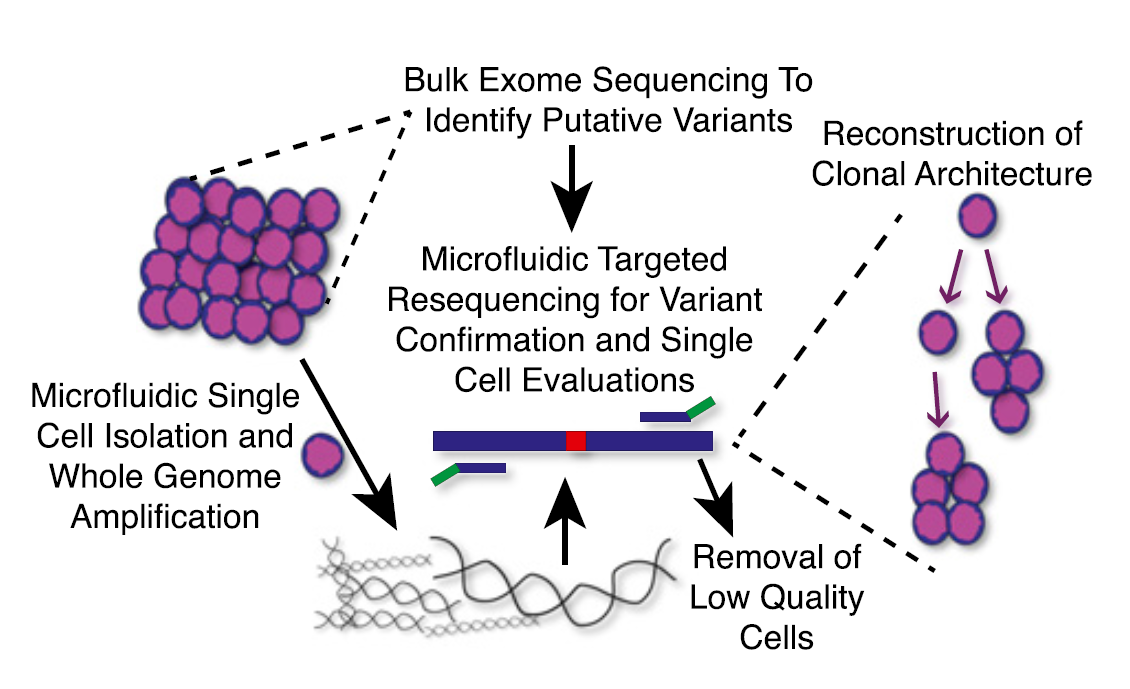
\includegraphics[scale=.2]{03.png}
		{\tiny Gawad et al, PNAS, 2014}
	\end{figure}
\end{frame}

\begin{frame}{Computational Methods}

	Combined \textbf{probabilistic} and \textbf{clustering} approach

	\begin{figure}
		\center
		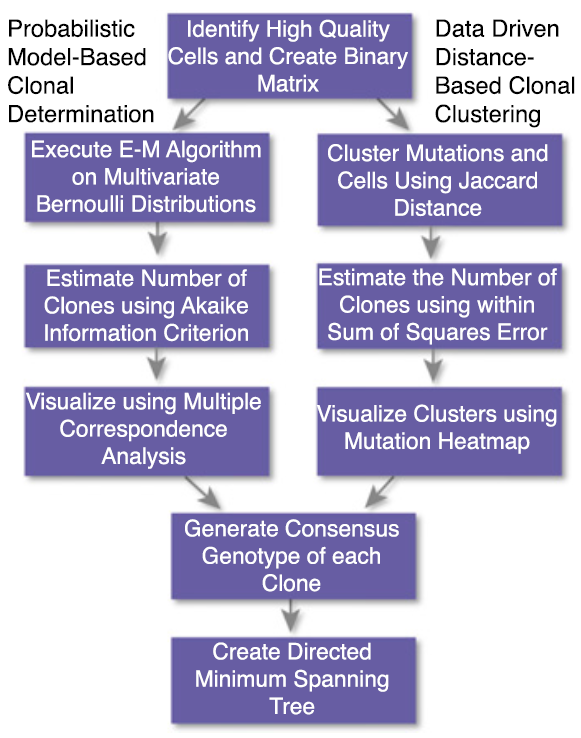
\includegraphics[scale=.3]{04.png}
		{\tiny Gawad et al, PNAS, 2014}
	\end{figure}
\end{frame}

\begin{frame}{Probabilistic Approach}
	
	Define:
	\begin{itemize}
		\item Vector representation of an individual's single-cell mutational profile $\mathbf{x} := (x_1, x_2, \cdots x_d)$ with $x_i \in \{0, 1\}$ denoting presence of mutation at i-th base.
		\item Probability of observing mutation $\theta_i = P(x_i = 1)$
	\end{itemize}
	
	We can model mutation as Bernoulli process and hence arrive at following probability of single-cell mutational profile $x$:
	
	
	$$P(\mathbf{x}|\Theta) = P(x_1, \cdots, x_d|\Theta) = \prod_{i=1}^{d} \theta_i^{x_i}(1 - \theta_i)^{1 - x_i}$$
	
	(This is the model for only one clone, i.e. single lineage)
	
\end{frame}

\begin{frame}
	For different clones $c_1, \cdots c_J$ with $\pi_j$ the proportion of j-th clone and $\sum_{j=1}^J \pi_j = 1$ we can represent the probability as finite mixture of multivariate Bernoulli distribution \textbf{for each cell}:
	
	$$P(\mathbf{x}|\Theta) = \sum_{j=1}^{J} \pi_j P(\mathbf{x} | \Theta_j) = \sum_{j=1}^{J} \pi_j \prod_{i=1}^{d} \theta_{ji}^{x_i}(1 - \theta_{ji})^{1 - x_i}$$
	
	The probability for N cells are then:
	
	$$P(\mathbf{x^{(1)}, \cdots, x^{(N)}}|\Theta) = \prod_{n=1}^{N} (\sum_{j=1}^{J} \pi_j \prod_{i=1}^{d} {\theta_i}^{x_{ni}}(1 - \theta_{ji})^{1 - x_{ni}} )$$	
	
	The log-likelihod of parameters $\{\pi_j, \Theta_j\}_{j=1}^{J}$ can then be written as:
	
	$$l(\theta, \mathbf{\pi}) = \sum_{n=1}^{N} log( \sum_{j=1}^{J} \pi_j \prod_{i=1}^{d} {\theta_i}^{x_{ni}}(1 - \theta_{ji})^{1 - x_{ni}})$$
\end{frame}

\begin{frame}{Probabilistic Approach -- Expectation Maximization}
	Estimation of clone membership of each cell using \textbf{Expectation Maximization (EM)}:
	
	\begin{enumerate}
		\item \textbf{Estimation step}: assign the clone category weights for each cell using the likelihood $l(\theta, \mathbf{\pi})$, i.e. $E[\mathbf{c}|l]$
		\item \textbf{Maximization step}: maximize the likelihood to get new $\theta$ \& clone proportion estimate based on estimated weights, i.e. $argmax_{\{\theta, \pi_1 \cdots \pi_N\}}\{l(\theta, \mathbf{\pi})\}$
		\item Repeat steps 1 \& 2 until the parameters converge
	\end{enumerate}	 
	
	\begin{figure}
		\center
		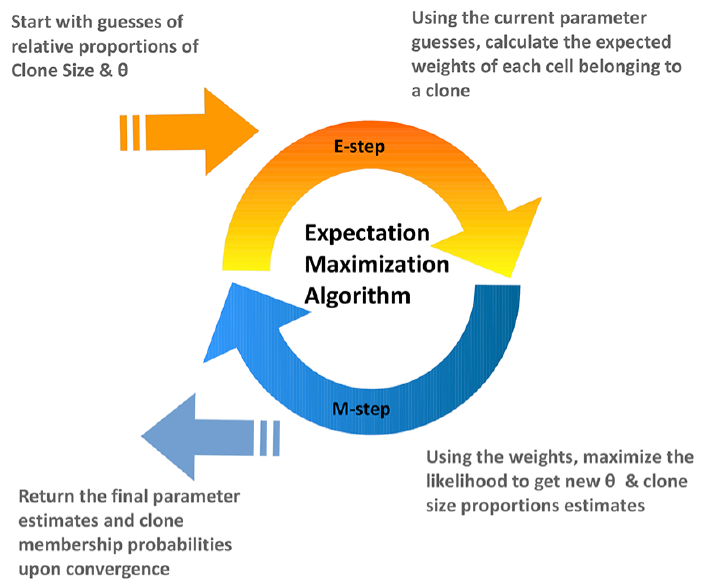
\includegraphics[scale=.3]{05.png}
		{\tiny Gawad et al, PNAS, 2014}
	\end{figure}
\end{frame}

\begin{frame}{Probabilistic Approach -- BIC}
	\begin{itemize}
		\item During EM step, models with larger number of clones are preferred:
			$$l(\theta, \mathbf{\pi}) = \sum_{n=1}^{N} log( \sum_{j=1}^{J} \pi_j \prod_{i=1}^{d} {\theta_i}^{x_{ni}}(1 - \theta_{ji})^{1 - x_{ni}})$$
		\item Overfitting is done by introducing BIC (Bayesian Information Criterion), which would penalize models with more free parameters:
			$$BIC = ln(N)J - 2 ln(l)$$
	\end{itemize}
	Upon this, each cell will be assigned to respective clonal population given the model and observed data.
\end{frame}

\begin{frame}{Probabilistic Approach -- Multiple Correspondence Analysis (MCA)}
	MCA $\sim$ Principal Component Analysis (PCA) on categorical data:
	
	\begin{itemize}
		\item Representation of the cells in two-dimensional space allows the validation of clone assignment
	\end{itemize}
	
	\begin{figure}
		\center
		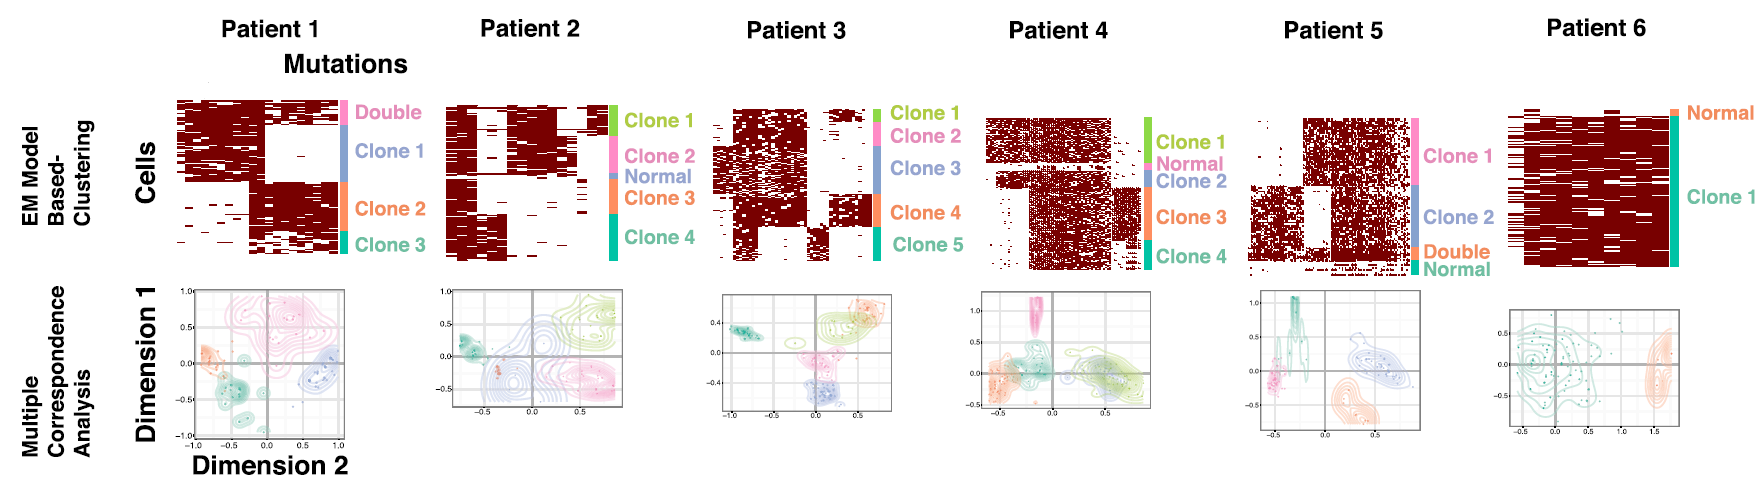
\includegraphics[scale=.3]{06.png}
		{\tiny Gawad et al, PNAS, 2014}
	\end{figure}
\end{frame}

\begin{frame}{Clustering Approach -- Clustering on Jaccard Distance}

		$$J(\mathbf{x_1}, \mathbf{x_2}) = \frac{|\{x_i | x_{1i} = 1 \wedge x_{2i} = 1 \}|}{|x_1|}$$
	
	\begin{itemize}
		\item Hierarirchal clustering over the distances reveals tree-structured relations among cells.
		\item Number of clones is estimated using sum of square error of elements in a cluster (Ward's method)
	\end{itemize}
	
	\begin{figure}
		\center
		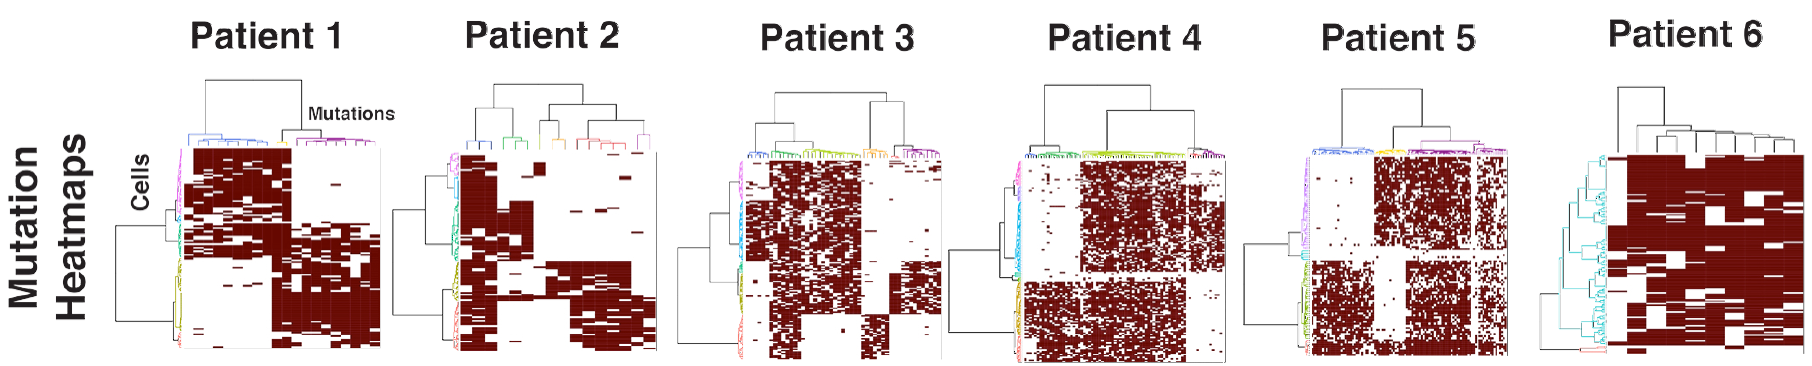
\includegraphics[scale=.2]{07.png}
		{\tiny Gawad et al, PNAS, 2014}
	\end{figure}
\end{frame}

\begin{frame}{Combined Approach}

	\begin{itemize}
		\item Clonal assignment results from both approaches are combined to show validity.
		\item Clones genealogy inferrence is done by introducing temporal ordering of the cells and applying Maximum Parsimony method (Farris, 1970 \& Fitch, 1971).
	\end{itemize}
	
	\begin{figure}
		\center
		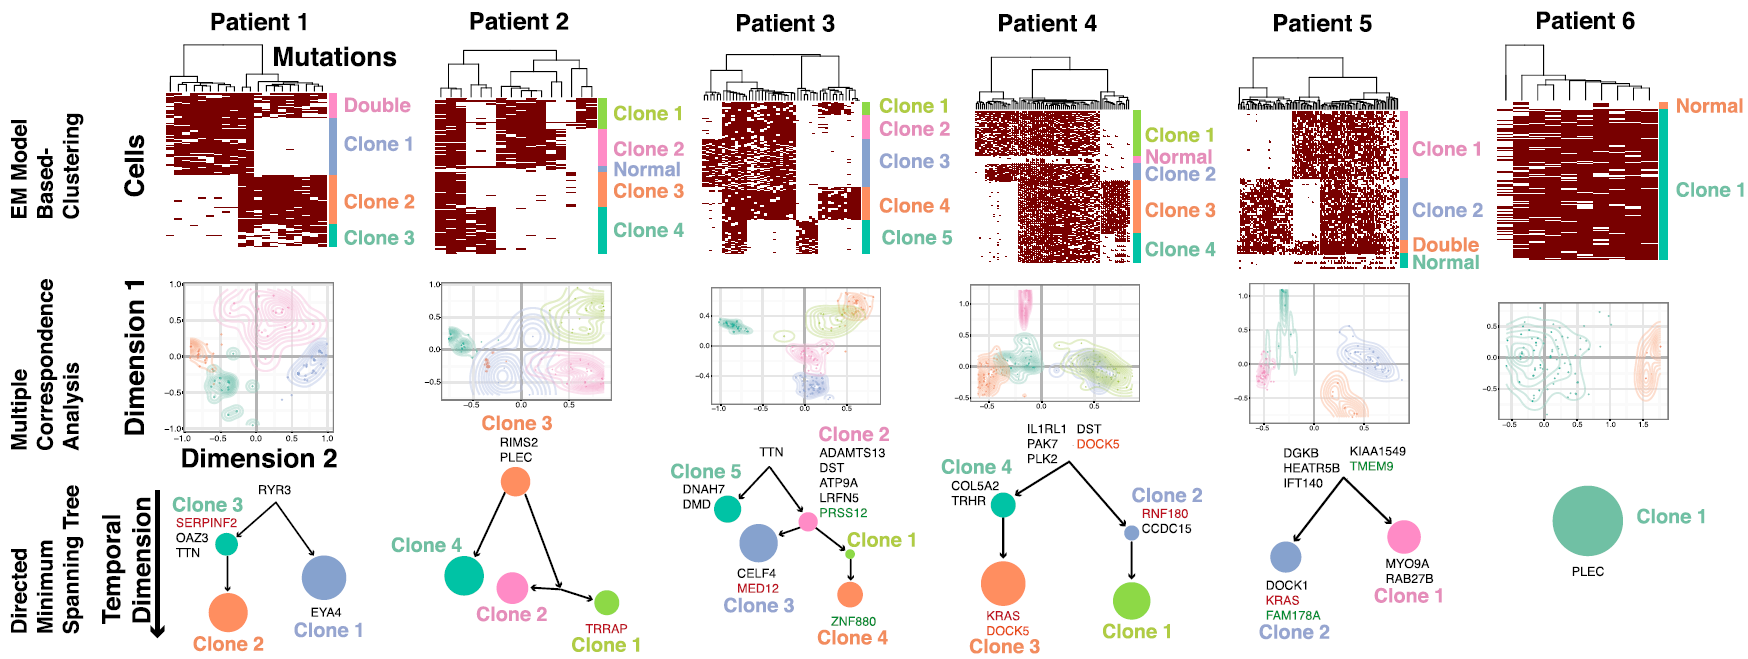
\includegraphics[scale=.2]{08.png}
		{\tiny Gawad et al, PNAS, 2014}
	\end{figure}
\end{frame}

\begin{frame}{Code Session}
	Data and code repo: \href{http://github.com/lianchye/Clonal_Analysis.git}{github.com/lianchye/Clonal\_Analysis.git}
\end{frame}

\begin{frame}{Paper review}
	\begin{itemize}
		\item \textbf{Readability:} 4 -- paper is overal readable
		\item \textbf{Reproducibility:} 5 -- github repo!
		\item \textbf{Novelty:} 3 -- simple and yet powerful method to identify intratumor heterogeneity
		\item \textbf{Impact:} 4 -- usable for other cancer classes
		\item \textbf{Aesthetics:} 3 -- aesthetic okay, some typos in appendix
		\item \textbf{Structure:} 2 -- personally more interested in methods and less in tiny detailed results
		\item \textbf{Overall:} 4 -- good paper
	\end{itemize}
\end{frame}


\begin{frame}{References}
	\begin{itemize}
		\item Gawad, Charles, Winston Koh, and Stephen R. Quake. "Dissecting the clonal origins of childhood acute lymphoblastic leukemia by single-cell genomics." Proceedings of the National Academy of Sciences 111.50 (2014): 17947-17952.
		\item Kandoth, Cyriac, et al. "Mutational landscape and significance across 12 major cancer types." Nature 502.7471 (2013): 333-339.
		\item Swanton, Charles. "Intratumor heterogeneity: evolution through space and time." Cancer research 72.19 (2012): 4875-4882.
		\item Ward Jr, Joe H. "Hierarchical grouping to optimize an objective function." Journal of the American statistical association 58.301 (1963): 236-244.
		\item Farris, James S. "Methods for computing Wagner trees." Systematic Biology 19.1 (1970): 83-92.
	\end{itemize}
\end{frame}


\end{document}